\documentclass{article}

% neurips_2026.sty loads natbib itself; options must be passed before it.
% "numbers" keeps the bracketed numeric citation style, e.g. [1].
\PassOptionsToPackage{numbers}{natbib}

% Workshop track, camera-ready (Interpretability as a Science @ NeurIPS 2026).
% "final" de-anonymizes and sets the footer to the workshop track name.
\usepackage[dblblindworkshop,final]{neurips_2026}
\workshoptitle{Interpretability as a Science}

% to avoid loading the natbib package, add option nonatbib:
%    \usepackage[nonatbib]{neurips_2026}

\usepackage[utf8]{inputenc} % allow utf-8 input
\usepackage[T1]{fontenc}    % use 8-bit T1 fonts
\usepackage{hyperref}       % hyperlinks
\usepackage{url}            % simple URL typesetting
\usepackage{booktabs}       % professional-quality tables
\usepackage{amsfonts}       % blackboard math symbols
\usepackage{amsmath}        % math environments
\usepackage{nicefrac}       % compact symbols for 1/2, etc.
\usepackage{microtype}      % microtypography
\usepackage{xcolor}         % colors
\usepackage{graphicx}       % figures
\hypersetup{hidelinks}      % keep cross-references unobtrusive in print

\title{When Do Attention-Head Ablations Support Causal Claims? \\
Projection-Level Confounds, Floor Effects, and Matched Controls}

\author{%
  Juli Huang \\
  Stanford University \\
  \texttt{julih@stanford.edu}
}


\begin{document}


\maketitle


\begin{abstract}
Attention-head ablation, replacing a head's output and measuring the
resulting change in task performance, is a standard way to infer which
components of a language model are causally responsible for a behavior.
Using GPT-2 small as a case study, with replications on DistilGPT2 and
Qwen2.5-1.5B-Instruct, we show that this recipe is fragile in ways that
are rarely checked. First, a natural implementation of ``zero out head
$h$'' (overwriting a channel slice of the attention block's
\emph{returned} output) does not ablate a single head, because the
output projection has already mixed all heads. On a controlled
induction-style copying task, this naive method is essentially
uncorrelated with a corrected, pre-projection ablation (Pearson
$r=0.057$) and selects a disjoint top-5 set of heads. The confound
recurs on both other models. Second, accuracy cannot register further
degradation at a floor (0.0\% on an off-target arithmetic task) and can
miss confidence changes near a ceiling (99.5\% on copying), while
log-probability stays graded. Third, with a discovery/held-out split and
1{,}000 matched random-head and layer-matched control draws, the top-5
selected heads' held-out effect exceeds both controls (Monte Carlo
$p=0.001$), and it does so in all 20 random re-partitions. That effect,
however, depends on the replacement value: the same GPT-2 heads' effect
falls from 0.412 nats to 0.005 under mean-ablation and to 0.020 under
resample-ablation, and on indirect object identification zero-ablation
shares only 2 of its top-5 heads with mean or resample ablation. Task specificity is not established on
GPT-2: the contrast with arithmetic is inconclusive ($p=0.078$;
$p=0.274$ at $N=500$), and against a format-matched sequence-continuation
control it disappears ($p=0.567$). A single-head ablation result is not
self-certifying. It requires verified projection semantics, a continuous
metric away from floor and ceiling, held-out matched controls, and a
stated replacement value checked against an on-distribution baseline.
\end{abstract}


\section{Introduction}
\label{sec:intro}

Interpretability researchers frequently ablate an individual attention
head, replacing its contribution and re-measuring task performance, and
interpret a resulting drop as evidence that the head is causally
responsible for some computation. Whether this inference is valid
depends on choices that are rarely audited: what, mechanically, gets
replaced relative to the attention block's linear mixing structure;
what it is replaced with; whether the evaluation metric has room to move
at all; and whether the identified heads are validated against an
appropriate null rather than just reported as the top of a ranking. This
paper asks a narrow, mechanical question: \textbf{under what conditions
does single-head ablation support a defensible causal interpretation},
in the sense of an effect that exceeds matched controls on held-out
data?

We answer it by auditing and fixing a head-ablation implementation,
designing a controlled induction-style copying task with behavioral
headroom alongside an off-target floor task and a format-matched control
task, and running a discovery/held-out pipeline with random and
layer-matched controls. The primary model is GPT-2 small (124M
parameters, 12 layers $\times$ 12 heads); DistilGPT2 and
Qwen2.5-1.5B-Instruct serve as replications, and indirect object
identification (IOI) on GPT-2 as an established circuit task. We report
four findings, one per research question (RQ0--RQ3), matching the
subsections of Section~\ref{sec:results}.

\textbf{(1, RQ0) The ablation implementation matters.} A hook registered on
the whole attention module's output, a natural way to write ``zero out
head $h$'', zeroes channels \emph{after} the block's output projection
has already mixed all heads together, so it does not isolate one head's
contribution. On our controlled copying task, this naive method's per-head effect
vector is essentially uncorrelated with a corrected, pre-projection
version (Pearson $r=0.057$), and the two methods' top-5 ``important''
heads share no head. The same holds on DistilGPT2 and Qwen2.5.

\textbf{(2, RQ1) Binary accuracy loses information at floor and near ceiling.} GPT-2
small scores 0.0\% on an off-target arithmetic task and 99.5\% on our
on-target copying task. At the floor, accuracy cannot register further
degradation. Near the ceiling, it can register a sufficiently large
drop but may hide confidence changes that leave the predicted token
unchanged. Teacher-forced log-probability of the gold continuation
remains graded in both regimes.

\textbf{(3, RQ2) With proper controls, five heads show a held-out-replicated
intervention effect that exceeds random and layer-matched baselines, but
their task specificity is not established on GPT-2.} The per-head
ranking is stable across splits (Spearman $\rho=0.974$ over all 144
heads), and the top-5 discovery-selected heads' mean held-out effect
clears both control distributions (Monte Carlo $p=0.001$ each), in the
original partition and in all 20 random re-partitions. Their contrast
against an off-target arithmetic task is inconclusive ($p=0.078$; $p=0.274$
in a pre-committed $N=500$ rerun), and against a format-matched
sequence-continuation task it disappears ($p=0.567$).

\textbf{(4, RQ3) The replacement value changes which heads are selected.}
Under mean-ablation and under resample-ablation, the five zero-selected
GPT-2 heads have almost no held-out effect (0.005 and 0.020 vs.\ 0.412
nats), and reselection yields sets that share no head with them. On IOI, zero-ablation shares only 2 of its top-5 heads
with mean or resample ablation. Baseline dependence is partial on
DistilGPT2 and small on Qwen2.5, so it must be checked per model.

Our contribution is a worked, fully reproducible example (code, seeds,
and every number traceable to a saved result file) showing that a
positive \emph{or} null single-head ablation result is not
self-certifying: a causal interpretation additionally requires (i)
verifying the intervention's projection semantics, (ii) a continuous
metric that is not saturated, (iii) matched controls evaluated on
data not used for head selection, and (iv) a stated replacement value
checked against at least one on-distribution baseline.


\section{Why naive head ablation can mislead}
\label{sec:background}

GPT-2's attention block computes a per-head output for each head,
concatenates the per-head outputs, and applies a single dense output
projection ($W_O$, \texttt{c\_proj} in the standard \texttt{transformers}
implementation) before adding the result to the residual stream.
\citet{elhage2021framework} describe $W_O$ as half of each
head's output-value (OV) circuit. Because $W_O$ spans the concatenated head dimension,
each output channel can receive contributions from all heads.
A hook that zeroes a contiguous, head-sized slice of the block's
\emph{returned} output (registered as a forward hook on the whole
attention module) therefore does not remove one head's contribution. It
removes an arbitrary linear combination of all heads' contributions to a
subset of output channels, after mixing has already happened. The
correct intervention instead zeroes the corresponding slice of $W_O$'s
\emph{input}, i.e., the concatenated, not-yet-mixed per-head values,
which requires a pre-hook on the projection itself rather than a
post-hook on the block.

We did not construct this as a strawman: it is the hook used by
this project's own original head-ablation implementation, which we
found when we audited it (preserved, unused for any reported result, as
\texttt{src/legacy\_invalid\_ablation.py}). We use it as
the ``naive'' method in our RQ0 comparison (Section~\ref{sec:results}).
The methods use the same nominal head index, model, and input. Their
activation interventions differ only in where they are applied within
the block.

\textbf{Scope of the failure.} The failure concerns an implementation
that treats a contiguous slice of the already-projected block output as
if it were one head. The confound is a property of where the
intervention is placed, not of a particular library. TransformerLens
\citep{nanda2022transformerlens} exposes a per-head, pre-projection hook
(\texttt{hook\_z}), which corresponds to our valid intervention, but it
also exposes the block's mixed output (\texttt{hook\_attn\_out}), where
slicing channels would reproduce the naive method. NNsight
\citep{fiottokaufman2025nnsight} exposes both the output of an attention
module and the input of its output projection, so the same choice arises
there. Our results do not show that these libraries implement the error,
and we did not measure how often the naive placement occurs in published
work. They show that the semantics of an intervention must be checked
against the model's computational graph.

\textbf{Choice of replacement value.} Zero-ablation sets a head's output
to a value it may never take during normal operation. Circuit analyses
therefore often replace activations with dataset means
\citep{wang2023interpretability}, and \citet{li2024optimal} propose
optimal ablation as an alternative. We use zero-ablation for the primary
analysis because it is a common default, and we test whether the
conclusions survive mean and resample replacement in
Sections~\ref{sec:mean}--\ref{sec:ioi}.

Separately, prior work has repeatedly cautioned that single-component
interventions and attention weights are easy to over-interpret without
controls: \citet{jain2019attention} show attention
weights alone are often uncorrelated with feature importance, and
\citet{michel2019sixteen} show many heads can be pruned
post hoc without hurting overall performance, i.e., that a head being
prunable does not mean it was doing nothing task-specific. More recent
circuit-style work explicitly validates causal claims about specific
components against matched baselines and held-out data
\citep{meng2022locating,wang2023interpretability,conmy2023towards}. Our contribution is
narrower and more mechanical: we isolate the projection-level
implementation confound specifically, and combine it with a
floor/ceiling-aware metric and a minimal control battery in one
end-to-end worked example.


\section{Experimental design}
\label{sec:design}

\textbf{Models.} The primary model is GPT-2 small (124M parameters, 12
layers, 12 heads/layer, 144 heads total), the standard Hugging Face
\texttt{transformers} implementation (v4.57.3, torch~2.8.0), run on CPU.
Replications use DistilGPT2 (6 layers, 72 heads), which is distilled from
GPT-2 and therefore not an independent architecture, and
Qwen2.5-1.5B-Instruct \citep{qwen2025qwen25} (28 layers, 12 query heads
per layer, 336 heads), whose output projection is hooked in the same
pre-projection position.

\textbf{Tasks.} \emph{Controlled induction-style copying} (target task, expected
headroom): synthetic four-word sequences of the form ``$w_1\ w_2\ w_3\
w_4$ . $w_1\ w_2\ w_3$'' $\to$ ``\ $w_4$'', with $w_1,\dots,w_4$ drawn
without replacement from a pool of common English words verified to
tokenize as exactly one byte-pair-encoding (BPE) token, a minimal instance of the
induction-head phenomenon described by
\citet{olsson2022induction} and traced to two-layer head
composition by \citet{elhage2021framework}. We generated
$N=200$ examples (seed 0) and split them 50/50 into a \emph{discovery}
set (used only to select candidate heads) and a \emph{held-out} set
(used only to evaluate them), fixed before any head effect was computed.
\emph{Arithmetic} (off-target control task): ``Q: $a$+$b$='' $\to$ ``\
$a{+}b$'', $a,b$ drawn uniformly from $[1,20]$, $N=200$ (seed 1), used
only to test task-specificity of already-selected heads, never for
selection. \emph{Ordered-sequence continuation} (format-matched control
task, added for the camera-ready version): ``$x_1\ x_2\ x_3\ x_4$ .
$x_5\ x_6\ x_7$'' $\to$ ``\ $x_8$'', where $x_1,\dots,x_8$ are eight
consecutive items of a familiar ordering (numerals 1--99, months, capital
letters, number words one--twenty). Every non-wrapping window is used
once, giving $N=129$ examples (92 numerals, 19 letters, 13 number words,
5 months). The template, the period, and the single-token,
space-prefixed answer match the copying task, but the answer never
appears in the prompt, so it cannot be copied in context. It is
predicted from knowledge of the ordering, a behavior attributed to
``successor heads'' \citep{gould2024successor}. Every generated example is checked so that the question's
tokenization is an exact token-level prefix of question+answer (BPE
merges are not always prefix-stable across concatenation). Examples
failing this check are dropped (and, for the two sampled tasks,
regenerated).

\textbf{Choice of tasks.} The tasks are deliberately simple. We use them
to isolate methodological issues in head ablation, not to benchmark
language understanding. Copying gives a predictable continuation with
behavioral headroom. Arithmetic is an off-target diagnostic that also
exposes accuracy at a floor, and it is not a matched control: it differs
from copying in template, computation, answer tokenization, and baseline
performance. The sequence task is a matched control in template,
answer length, and baseline (Section~\ref{sec:rq2}). Simple tasks make
the diagnostic results interpretable, but they limit conclusions about
more complex behaviors, so we also test an established circuit task,
indirect object identification (Section~\ref{sec:ioi}).

\textbf{Metrics.} \emph{Teacher-forced exact match}: the greedy argmax
token at every answer position must equal the gold token (binary).
\emph{Teacher-forced log-probability}: $\sum_t \log p(\text{gold
token}_t \mid \text{prefix})$ over the answer's tokens (continuous,
natural log). Both require a single forward pass per batch (no
autoregressive generation).

\textbf{Ablation methods.} \texttt{naive\_post\_projection}: a forward
hook on the attention module's output, zeroing a head-sized channel
slice of the returned (already-projected) tensor. This is invalid and
used only for the RQ0 comparison. \texttt{head\_ablation}: a forward
pre-hook on the output projection's input, zeroing the corresponding
pre-mix slice. Every causal claim uses this pre-projection location.
The primary analysis replaces the slice with zero. The robustness checks
replace it with the slice's mean (\emph{mean-ablation}; computed over all
non-padding positions of the discovery split only and applied unchanged
to every split, so held-out data never inform the intervention) or with
its activation on another input (\emph{resample-ablation}). For copying,
the source is a different example from the same split whose words split
into the same numbers of tokens, so every position plays the same role
(one discovery example has no such partner and is dropped, leaving 99);
for IOI, it is a corrupted prompt (Section~\ref{sec:ioi}). These semantics are asserted by
executable tests that run before the pipeline and ship with the code: on a
small GPT-2 configuration they check that the pre-hook zeroes exactly the
requested head's slice of the projection input and leaves every other
channel unchanged, that removing the hook exactly restores the unablated
output, and that the naive hook alters the logits while leaving that
projection input untouched.

\textbf{Head selection.} For all 144 heads, we compute the mean
$\Delta = \overline{\text{log-prob}}_{\text{baseline}} -
\overline{\text{log-prob}}_{\text{ablated}}$ over a data split, using
one batched forward pass per head (not per example). Candidate heads
are the top-5 by $\Delta$ on the discovery split only.

\textbf{Controls.} \emph{Random-head control}: 1{,}000 draws of 5 heads
sampled uniformly without replacement from all 144. \emph{Layer-matched
control}: 1{,}000 draws that preserve the candidate set's size and layer
composition while replacing every candidate identity, drawing each
layer's replacements without replacement from that layer's
non-candidate heads. Both exclusions matter whenever one layer supplies
several candidates, as ours does: replacing each candidate independently
would let a single head stand in for several candidates, and would let a
candidate head enter its own control distribution. Both controls are
built by resampling the already-computed 144-head $\Delta$ vector, so
they cost no additional forward passes. These two controls ask whether
the candidates' effect is unusual \emph{among heads}. A separate
\emph{specificity} contrast asks whether it differs \emph{between
tasks}: the candidates' held-out copying $\Delta$ minus their $\Delta$ on
a control task, compared with the same quantity for the 1{,}000 random
head sets. Passing the head controls does not imply passing the task
contrast.

\textbf{Statistics.} Where applicable, example-level point estimates are
reported with percentile-bootstrap 95\% confidence intervals (CIs;
2{,}000 resamples over examples). Control ranges are the 5th--95th
percentiles of 1{,}000 draws. One-sided Monte Carlo $p$-values use the
finite-sample correction $(k+1)/(B+1)$, where $k$ of $B=1{,}000$ control
draws match or exceed the candidate statistic. Rank stability across
splits is measured with Spearman correlation over all 144 heads.

\textbf{Reproducibility.} Seeds (induction generation~0, arithmetic
generation~1, control sampling~42), package versions, and the experiment
configuration are recorded with every saved result. The full pipeline
(\texttt{scripts/run\_neurips\_experiments.py}) reruns end-to-end in
198.99~s for the primary GPT-2 configuration on one 10-core Apple M5 CPU
with 24~GB unified memory and no GPU (peak resident memory 1.94~GiB),
57.62~s for DistilGPT2, and 428.56~s for GPT-2 at $N=500$ (3.22~GiB).
Each of the three configurations was then rerun independently; all three
reproduced their saved result files exactly, byte for byte, apart from
the recorded timestamp. The camera-ready partition and sequence-control
analyses (\texttt{scripts/run\_camera\_ready\_robustness.py}) took
301.43~s (1.90~GiB) for GPT-2 and 82.08~s (1.63~GiB) for DistilGPT2,
and the copying resample analysis
(\texttt{scripts/run\_resample\_copying.py}) took 914.99~s (2.14~GiB)
and 325.98~s (2.10~GiB).
The software environment, model revisions,
file hashes, storage, and verification commands are recorded in
\texttt{neurips/experiment\_results/reproducibility\_provenance.md}. Every
number in this paper is read from a result JSON file, and a script
(\texttt{scripts/verify\_paper\_numbers.py}) checks the printed values
against those files.


\section{Results}
\label{sec:results}

\subsection{RQ0: Does the ablation implementation matter?}
\label{sec:rq0}

On the controlled copying-task discovery split, the naive and correct per-head
$\Delta$ vectors are nearly uncorrelated (Pearson $r=0.057$, Spearman
$\rho=0.110$; scatter plot in Appendix~\ref{app:rq0}), with a mean
absolute per-head disagreement of $0.067$ nats. The top-5 heads selected by each method share
\textbf{zero} heads. The same pattern holds on DistilGPT2 ($r=0.001$)
and on Qwen2.5-1.5B-Instruct ($r=0.108$, $\rho=0.176$), each with 0/5
top-head overlap (Appendices~\ref{app:distilgpt2} and~\ref{app:qwen}). The methods use the same nominal head index,
model, and input, but apply the activation intervention at different
points in the block (Section~\ref{sec:background}).
This is not a hypothetical failure mode: the naive intervention is a
natural, easy-to-write hook, and it is the one this project originally
used (Section~\ref{sec:background}), not one constructed to fail.

\subsection{RQ1: Metric behavior at floor and near ceiling}
\label{sec:rq1}

GPT-2 small is at a behavioral floor on the arithmetic control task
(0.0\% teacher-forced exact match, 95\% CI $[0.0\%, 0.0\%]$, $N=200$)
and near a behavioral ceiling on the controlled induction-style
copying task (99.5\%, CI $[98.5\%,100.0\%]$). At the floor, binary
accuracy cannot detect further degradation. Near the ceiling, it can
detect a sufficiently large damaging effect, but a substantial
confidence decrease may leave every argmax prediction unchanged. Log-probability
remains graded: mean log-prob is $-7.44$ nats (CI
$[-7.53,-7.35]$) on arithmetic and $-0.83$ nats (CI $[-0.90,-0.76]$) on
the copying task (Table~\ref{tab:main}, Figure~\ref{fig:main}A), and, as shown
next, individual-head
ablation moves it substantially and reproducibly. This is why we select
and validate candidate heads using log-probability rather than accuracy
throughout. A post hoc check of one alternative answer format shows that
the GPT-2 floor is not an artifact of the leading space in the gold
answer: exact match remains 0.0\% when the answer is written without it.
This is not true for every model. Qwen2.5-1.5B-Instruct also scores
0.0\%, because its tokenizer splits ``\ 24'' into a bare space token
followed by digits and the model never predicts the bare space. Without
the space it scores 23.0\% (Appendix~\ref{app:qwen}). A floor in
accuracy can therefore reflect the answer format rather than missing
capability. Log-probability stays graded in either case (Qwen2.5:
$-5.31$ nats).

\subsection{RQ2: Specificity of selected-head intervention effects}
\label{sec:rq2}

The top-5 discovery-selected heads are Layer~0 Head~0, Layer~0 Head~7,
Layer~1 Head~3, Layer~11 Head~0, and Layer~0 Head~10 (four in the first
two layers, one in the last layer). Two distinct pieces of evidence
support them. First, the per-head effect ranking is highly stable across
the discovery and held-out splits (Spearman $\rho=0.974$ over all 144
heads), so head ordering is not an artifact of the discovery sample.
Second, the candidates' mean held-out effect, $0.412$ nats (CI
$[0.353,0.474]$), is far outside both the matched random-head control
distribution (mean $0.029$, 5th--95th percentile range
$[-0.033,0.113]$; Monte Carlo $p=0.001$,
0/1{,}000 draws matched or exceeded the candidates) and the
layer-matched control distribution (mean $0.051$, 5th--95th percentile
range $[0.001,0.098]$;
Monte Carlo $p=0.001$; Figure~\ref{fig:main}B). This establishes a held-out-replicated
intervention effect on the controlled copying task that exceeds what an arbitrary
head, or an arbitrary head from the same layers, would produce. Whether
that effect is specific to the copying task requires the separate contrast below.

Task specificity is not established (Figure~\ref{fig:main}C). The
specificity statistic (held-out copying-task $\Delta$ minus
arithmetic-control $\Delta$) is $0.139$ nats for the candidates, versus a
random-control distribution with mean $0.011$ and 5th--95th percentile
range $[-0.135,0.165]$ (Monte Carlo $p=0.078$). A single pre-committed
rerun with $N=500$ per task preserves the held-out effect over both head
controls ($p=0.001$ each) but weakens the contrast to $0.056$ nats
($p=0.274$). We therefore treat the arithmetic contrast as inconclusive.
Even a significant contrast against arithmetic would be hard to
interpret, because the two tasks differ in template, computation,
tokenization, and baseline performance.

\textbf{A format-matched control removes the GPT-2 contrast.} We
therefore added the ordered-sequence task (Section~\ref{sec:design}),
whose template, answer length, and baseline match copying (GPT-2: 96.9\%
exact match, $-0.57$ nats) but whose answer cannot be copied from the
prompt. This analysis and the partition analysis below were specified
in writing before they were run and are reported as run. Ablating the
five GPT-2 candidates lowers the sequence-task log-probability by 0.447
nats, far more than random head sets do (mean 0.051, $p=0.001$) and as
much as it lowers held-out copying. Their specificity against this
control is $-0.035$ nats (random-control mean $-0.023$, $p=0.567$), and
the candidates selected under mean-ablation (Section~\ref{sec:mean})
behave the same way ($-0.138$ nats, $p=0.882$). On GPT-2, we therefore find no evidence
under either baseline that the selected heads' effect is specific to
in-context copying: they harm the format-matched task at least as much.
A null contrast against one control task does not, however, rule out
specificity relative to other tasks.
DistilGPT2 differs. Its candidates lower the sequence task by only 0.113
nats, no more than random head sets (mean 0.107, $p=0.280$), so their
specificity is 0.472 nats ($p=0.001$; mean-ablation candidates 0.382,
$p=0.001$). For DistilGPT2, the effect is larger on in-context copying
than on a format-matched task that cannot be solved by copying. This is
evidence of a task-dependent effect, not of an induction mechanism. The
baseline match is also looser for DistilGPT2 (87.6\% exact match on the
sequence task vs.\ 90.0\% on copying).

\textbf{Sensitivity to the partition.} We repeated selection and
evaluation over 20 random 100/100 partitions of the 200 copying examples
(Appendix~\ref{app:partitions}). On GPT-2, the same five candidates are
selected in 19 of 20 partitions and exceed both head controls in all 20
($p=0.001$), with a median held-out effect of 0.441 nats (range
0.368--0.469). The arithmetic specificity contrast, however, gives
$p\le0.05$ in 9 of 20 partitions (median $p=0.054$), so whether it
crosses the conventional threshold depends on the partition. On
DistilGPT2, the same five heads are selected in all 20 partitions, and
both head controls and the arithmetic contrast give $p=0.001$ in each.
The partitions overlap, so this is a sensitivity analysis rather than 20
independent replications.

\begin{table}[t]
  \caption{Primary GPT-2 RQ1/RQ2 quantities. All values are computed
  from \texttt{gpt2\_results.json} (Section~\ref{sec:design}). CIs are
  95\% percentile bootstrap over examples except where noted.
  ``Control range'' is the 5th--95th percentile of 1{,}000 control
  draws, not a CI.}
  \label{tab:main}
  \centering
  \small
  \begin{tabular}{lrrl}
    \toprule
    Quantity & Value & Interval & $N$ / draws \\
    \midrule
    Copying-task accuracy (ceiling) & 0.995 & [0.985, 1.000] & 200 \\
    Arithmetic accuracy (floor) & 0.000 & [0.000, 0.000] & 200 \\
    Copying-task log-prob (nats) & $-0.83$ & [$-0.90$, $-0.76$] & 200 \\
    Arithmetic log-prob (nats) & $-7.44$ & [$-7.53$, $-7.35$] & 200 \\
    Candidate $\Delta$, held-out & 0.412 & [0.353, 0.474] & 100 \\
    Random-control $\Delta$, held-out & 0.029 & [$-0.033$, 0.113]$^\dagger$ & 1000 \\
    Layer-matched $\Delta$, held-out & 0.051 & [0.001, 0.098]$^\dagger$ & 1000 \\
    Rank stability (disc.\ vs.\ held-out, $\rho$) & 0.974 & -- & 144 heads \\
    Candidate specificity & 0.139 & -- & -- \\
    Random-control specificity & 0.011 & [$-0.135$, 0.165]$^\dagger$ & 1000 \\
    \bottomrule
  \end{tabular}
  \vspace{0.3em}
  \\
  \raggedright \footnotesize Monte Carlo $p$(candidate $\geq$ random control, held-out $\Delta$) $=0.001$; \quad
  $p$(candidate $\geq$ layer-matched, held-out $\Delta$) $=0.001$; \quad
  $p$(candidate $\geq$ random control, specificity) $=0.078$. $^\dagger$5th--95th percentile.
\end{table}

\begin{figure}[t]
  \centering
  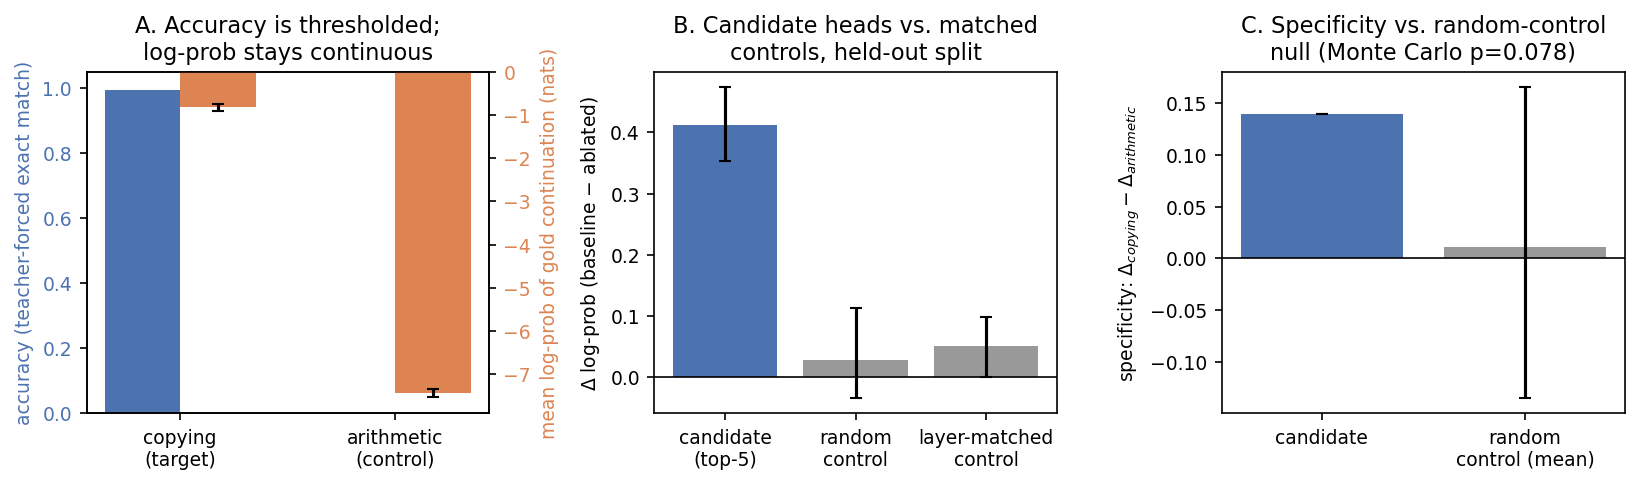
\includegraphics[width=\linewidth]{figures/main_figure.png}
  \caption{\textbf{A.} Accuracy cannot show further degradation at the
  arithmetic floor and may hide confidence changes near the copying-task
  ceiling. Log-probability stays continuous.
  \textbf{B.} The top-5 candidate heads' held-out effect far exceeds
  matched random-head and layer-matched control distributions (error
  bars: 95\% CI for the candidate, 5th--95th percentile for controls).
  \textbf{C.} Specificity (copying minus arithmetic effect) is larger
  for candidates than the random-control mean, but the contrast is
  inconclusive (Monte Carlo $p=0.078$; $p=0.274$ at $N=500$) and
  disappears against a format-matched control
  (Section~\ref{sec:rq2}).}
  \label{fig:main}
\end{figure}


\subsection{RQ3: Does the replacement value change the conclusion?}
\label{sec:mean}

Zero is a value a head's output may never take, so the RQ2 effect could
reflect that distribution shift rather than the removal of a
computation. After obtaining the primary results, we therefore reran the
RQ2 pipeline with two replacement values that stay on the model's
activation distribution (Section~\ref{sec:design}): the head's mean output
(\emph{mean-ablation}) and its output on another copying example
(\emph{resample-ablation}, specified in writing before it was run). Data,
splits, selection rule, controls, seeds, and statistics are unchanged
(Table~\ref{tab:mean}).

\textbf{The protocol still finds heads that beat both controls.} Under
either baseline and on both models, the reselected candidates exceed the
random-head and layer-matched controls on held-out data (Monte Carlo
$p=0.001$ for each comparison). The matched-control protocol is
therefore not tied to zero-ablation.

\textbf{It finds different heads.} On GPT-2, the mean-ablation
candidates (Layer~10 Heads~11 and~0, Layer~7 Head~6, Layer~0 Heads~9
and~3) and the resample-ablation candidates (Layer~10 Heads~0, 11, 1,
and~6, Layer~11 Head~2) share no head with the zero-ablation candidates,
four of which lie in layers 0 and~1, but they share Layer~10 Heads~0
and~11 with each other. Per-head effects agree in the same way: on the
discovery split, mean- and resample-ablation correlate at Pearson
$r=0.724$, whereas zero-ablation correlates with them at only $0.424$
and $0.212$.

\textbf{The zero-selected heads lose their effect.} In a post hoc
comparison computed from the saved per-head effects, the five
zero-selected GPT-2 heads have a held-out effect of 0.005 nats under
mean-ablation instead of 0.412, below the mean of the mean-ablation
random control (0.016). Because a pooled mean is itself a value a head
may never produce, the pre-specified resample analysis tests the same
heads with replacements the heads actually produce. Their effect is
then 0.020 nats (CI $[0.006,0.035]$), no larger than that of random head
sets (mean 0.015, $p=0.346$) or layer-matched sets ($p=0.430$), and it
is 0.005 and 0.011 nats with two other random choices of source
examples. On GPT-2, the RQ2 effect of these heads is therefore
consistent with replacing their output by an off-distribution value, not
with removing information the copying task needs.

\textbf{How much the baseline matters depends on the model.} On
DistilGPT2, resample-ablation selects exactly the mean-ablation
candidates, which share one head with the zero-ablation set, and the
zero-selected heads keep about a third of their effect (0.586 nats under
zero, 0.182 under mean, 0.201 under resample). Under resample that
remainder exceeds layer-matched head sets ($p=0.001$) but not clearly
random ones ($p=0.075$). On Qwen2.5-1.5B-Instruct, mean-ablation
reselects the same five heads as zero-ablation, and they keep most of
their effect (0.208 to 0.155 nats; Appendix~\ref{app:qwen}); we did not
run resample-ablation on Qwen2.5.

\textbf{Task specificity does not return.} Under mean-ablation, the
GPT-2 candidates' contrast against arithmetic gives $p=0.014$ (0.168
nats versus a random-control mean of 0.021), but against the
format-matched sequence task the same candidates show no specificity
($p=0.882$; Section~\ref{sec:rq2}). We therefore do not read the
arithmetic result as evidence of task specificity.

\begin{table}[t]
  \caption{Robustness to the replacement value ($N=200$ per task; $\Delta$
  in nats). The first block compares per-head effects under zero and mean
  ablation. The second repeats RQ2 with candidates reselected under
  mean-ablation. The third evaluates the zero-selected candidates under
  zero and mean ablation and was computed post hoc from the saved per-head
  effects. The last block is the pre-specified resample-ablation analysis
  (discovery $N=99$, held-out $N=100$): held-out $\Delta$ of the stated
  heads, $p$-values against random and layer-matched head sets, and the
  per-head Pearson $r$ with the other two baselines on the discovery split. Intervals are 95\% percentile-bootstrap CIs over examples;
  $^\dagger$5th--95th percentile of 1{,}000 control draws.}
  \label{tab:mean}
  \centering
  \small
  \setlength{\tabcolsep}{4pt}
  \begin{tabular}{lrrrr}
    \toprule
    & \multicolumn{2}{c}{GPT-2 small} & \multicolumn{2}{c}{DistilGPT2} \\
    \cmidrule(lr){2-3} \cmidrule(lr){4-5}
    Quantity & Value & Interval & Value & Interval \\
    \midrule
    Zero vs.\ mean per-head $\Delta$: Pearson $r$ & 0.424 & -- & 0.553 & -- \\
    Zero vs.\ mean per-head $\Delta$: Spearman $\rho$ & 0.495 & -- & 0.871 & -- \\
    Top-5 overlap, mean- vs.\ zero-selected & 0/5 & -- & 1/5 & -- \\
    \midrule
    Candidate $\Delta$, held-out & 0.176 & [0.157, 0.194] & 0.445 & [0.388, 0.508] \\
    Random-control $\Delta$, held-out & 0.016 & [$-0.034$, 0.057]$^\dagger$ & 0.060 & [$-0.012$, 0.172]$^\dagger$ \\
    Layer-matched $\Delta$, held-out & 0.009 & [$-0.071$, 0.058]$^\dagger$ & 0.030 & [$-0.024$, 0.067]$^\dagger$ \\
    Rank stability $\rho$ & 0.948 & -- & 0.960 & -- \\
    $p$: random / layer-matched / specificity & \multicolumn{2}{r}{0.001 / 0.001 / 0.014} & \multicolumn{2}{r}{0.001 / 0.001 / 0.001} \\
    \midrule
    Zero-selected heads, held-out $\Delta$ under zero & 0.412 & -- & 0.586 & -- \\
    Zero-selected heads, held-out $\Delta$ under mean & 0.005 & -- & 0.182 & -- \\
    \midrule
    Zero-selected heads under resample & 0.020 & [0.006, 0.035] & 0.201 & [0.173, 0.232] \\
    \quad $p$: random / layer-matched & \multicolumn{2}{r}{0.346 / 0.430} & \multicolumn{2}{r}{0.075 / 0.001} \\
    Resample-selected, held-out $\Delta$ & 0.179 & [0.159, 0.200] & 0.586 & [0.516, 0.659] \\
    \quad $p$: random / layer-matched & \multicolumn{2}{r}{0.001 / 0.001} & \multicolumn{2}{r}{0.001 / 0.001} \\
    Overlap with zero / mean top-5 & \multicolumn{2}{r}{0/5 / 2/5} & \multicolumn{2}{r}{1/5 / 5/5} \\
    Pearson $r$ with zero / mean & \multicolumn{2}{r}{0.212 / 0.724} & \multicolumn{2}{r}{0.473 / 0.946} \\
    \bottomrule
  \end{tabular}
\end{table}

\subsection{RQ3 on an established circuit task: indirect object identification}
\label{sec:ioi}

To test whether baseline dependence also arises on a natural-language
circuit task, we ran indirect object identification (IOI;
\citealp{wang2023interpretability}) on GPT-2 small: 200 prompts from the
15 templates of \citet{wang2023interpretability} with single-token
names, places, and objects, a 100/100 discovery/held-out split, and the
logit difference between the indirect object and the subject as the
metric. GPT-2 prefers the indirect object on 97\% (discovery) and 100\%
(held-out) of prompts. We compared three replacement values at the same
pre-projection location: zero, the discovery-split mean, and a
\emph{resample} value, the head's activation on the ``ABC'' variant (the
second subject replaced by a third name) of a different prompt with the
same template. Selection, controls, and statistics are those of RQ2.

Under every baseline the selected heads exceed both matched controls
($p=0.001$ each). The baselines disagree on which heads matter: zero
shares only 2 of its top-5 heads with mean or with resample, whereas
mean and resample share 4 of 5 (Spearman $\rho$ over all 144 heads:
zero vs.\ mean $0.74$, zero vs.\ resample $0.47$, mean vs.\ resample
$0.65$). Zero-ablation selects three layer-0/1 heads that neither
on-distribution baseline selects, and its held-out effect is 68\% larger
(1.55 vs.\ 0.92 and 0.93). Under every baseline the top-5 includes the
S-inhibition heads 8.6 and 8.10 reported by
\citet{wang2023interpretability}, and their head 7.9 is in the top-5
under mean and resample (Appendix~\ref{app:ioi}).

\section{Discussion and limitations}
\label{sec:discussion}

\textbf{Scope of the causal claim.} We do not claim these five heads
``compute induction'' in a mechanistic sense. Using the causal-claim
ladder (correlation $<$ decodability $<$ intervention effect $<$
specific causal contribution $<$ mechanistic role), our evidence
supports a held-out-replicated intervention effect that exceeds matched
controls (the third rung), but only relative to a stated replacement
value. The zero-selected GPT-2 heads reach this rung under zero-ablation
and not under mean- or resample-ablation. The Qwen2.5 heads reach it under both. No
GPT-2 specificity contrast supports the fourth rung. A mechanistic
account would require further evidence, such as activation patching,
input-dependence analysis, or directional interventions.

\textbf{Task-control mismatch.} The arithmetic control differs from
copying in template, computational demands, tokenization, and baseline
performance, and it sits at an accuracy floor. A difference in ablation
effects between the two tasks therefore cannot be attributed uniquely to
a copying-specific computation, and we treat the arithmetic contrast as
a limited diagnostic. The sequence-continuation control
(Section~\ref{sec:rq2}) matches the template, answer length, and
baseline. It removes the GPT-2 contrast but not the DistilGPT2 one, and
it is still only one alternative rule.

\textbf{Ablation baseline.} We tested zero, mean, and resample
replacement (resample on copying for GPT-2 and DistilGPT2, and on IOI).
We did not test noise injection or optimal
ablation \citep{li2024optimal}, or resample-ablation on Qwen2.5. Because the baseline changed the selected
heads on GPT-2 and IOI but barely on Qwen2.5, whether it matters has to
be checked for each model and task.

\textbf{Model scope.} DistilGPT2 is distilled from GPT-2, so it is not an
independent replication. On it, the naive and correct effects are again
near-uncorrelated ($r=0.001$, 0/5 overlap), the arithmetic floor recurs,
and the selected heads exceed both matched controls
(Appendix~\ref{app:distilgpt2}). Copying accuracy is lower (90.0\%), so
the near-ceiling example is specific to GPT-2. Qwen2.5-1.5B-Instruct is
a different architecture family and reproduces the projection confound
and the matched-control separation (Appendix~\ref{app:qwen}). We did not
test models larger than 1.5B parameters, and the new partition,
sequence-control, and copying resample analyses were run on GPT-2 and
DistilGPT2 only, because
one Qwen pipeline run took 3.3 CPU-hours.

\textbf{Partitions and sample size.} The partition analysis reuses the
same 200 copying examples and uses zero-ablation only. The sequence
control has 129 examples, 92 of them numerals.

\textbf{Broader implication.} Each check changed a conclusion: the naive
hook selected disjoint heads; accuracy hid information at the floor and
near the ceiling; the specificity contrast blocked a task-specificity
claim that the larger GPT-2 run does not support; and the replacement
value changed which heads were selected and, for GPT-2, removed the
selected heads' effect under both on-distribution baselines. A single-head ablation report should therefore
state the intervention point with a test that it isolates one head, use
a continuous metric beside accuracy, select on held-out-separated data
against matched controls, and report the replacement value together with
at least one on-distribution baseline.


\section{Conclusion}
\label{sec:conclusion}

A head ablation is not self-certifying evidence of a specific causal role.
Hook placement can ablate the wrong quantity, accuracy is censored at a
floor and coarse near a ceiling, and held-out matched controls separate a
replicating effect from arbitrary disruption. That effect can still
depend on the replacement value, and task specificity can still fail to
replicate.


\bibliographystyle{unsrtnat}
{\small
\bibliography{references}
}

\newpage
\appendix

\section{Supplementary figure: RQ0 per-head comparison}
\label{app:rq0}

Figure~\ref{fig:rq0} plots the per-head effect (correct pre-projection
ablation vs.\ naive post-projection ablation) for all 144 heads on the
controlled copying-task discovery split, corresponding to the summary statistics in
Section~\ref{sec:rq0}.

\begin{figure}[h]
  \centering
  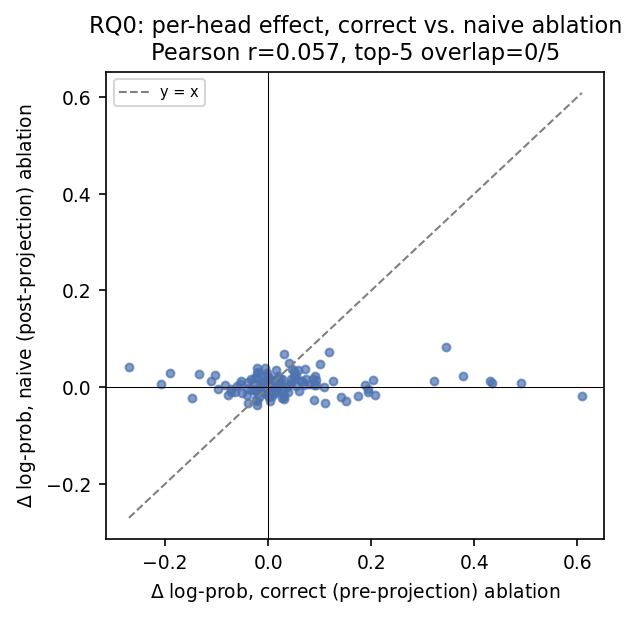
\includegraphics[width=0.6\linewidth]{figures/rq0_naive_vs_correct.png}
  \caption{Per-head $\Delta$ log-prob under the correct (pre-projection)
  vs.\ naive (post-projection) ablation method, all 144 heads,
  controlled copying-task discovery split. A valid replication of the naive method
  would lie near the $y=x$ line. Instead the two methods are nearly
  uncorrelated (Pearson $r=0.057$).}
  \label{fig:rq0}
\end{figure}

\section{Replication on a second model (DistilGPT2)}
\label{app:distilgpt2}

As a first robustness check (Section~\ref{sec:discussion}), we reran the identical pipeline
(Section~\ref{sec:design}), unchanged except for the model, on
DistilGPT2 (6 layers, 12 heads/layer, 72 heads total). All data,
metrics, ablation methods, splits, and control procedures are exactly
as in Section~\ref{sec:design}, and only the model differs. Results are in
Table~\ref{tab:distilgpt2}.

\begin{table}[h]
  \caption{DistilGPT2 replication of Table~\ref{tab:main}, with the same
  procedure and $N$s. The intervention-semantic and matched-control
  findings replicate, and the arithmetic floor recurs. Copying accuracy
  is lower (90.0\%), so GPT-2's near-ceiling example does not replicate.
  The specificity comparison gives Monte Carlo $p=0.001$.}
  \label{tab:distilgpt2}
  \centering
  \small
  \begin{tabular}{lrrl}
    \toprule
    Quantity & Value & Interval & $N$ / draws \\
    \midrule
    Copying-task accuracy & 0.900 & [0.855, 0.940] & 200 \\
    Arithmetic accuracy (floor) & 0.000 & [0.000, 0.000] & 200 \\
    Copying-task log-prob (nats) & $-0.96$ & [$-1.07$, $-0.85$] & 200 \\
    Arithmetic log-prob (nats) & $-7.38$ & [$-7.50$, $-7.25$] & 200 \\
    RQ0: Pearson $r$(naive, correct) & 0.001 & -- & 72 heads \\
    RQ0: top-5 head overlap & 0/5 & -- & -- \\
    Candidate $\Delta$, held-out & 0.586 & [0.511, 0.661] & 100 \\
    Random-control $\Delta$, held-out & 0.080 & [$-0.026$, 0.231]$^\dagger$ & 1000 \\
    Layer-matched $\Delta$, held-out & 0.054 & [$-0.017$, 0.128]$^\dagger$ & 1000 \\
    Rank stability ($\rho$, disc.\ vs.\ held-out) & 0.957 & -- & 72 heads \\
    Candidate specificity & 0.492 & -- & -- \\
    Random-control specificity & 0.023 & [$-0.159$, 0.222]$^\dagger$ & 1000 \\
    \bottomrule
  \end{tabular}
  \vspace{0.3em}
  \\
  \raggedright \footnotesize Monte Carlo $p$(candidate $\geq$ random control, held-out $\Delta$) $=0.001$; \quad
  $p$(candidate $\geq$ layer-matched, held-out $\Delta$) $=0.001$; \quad
  $p$(candidate $\geq$ random control, specificity) $=0.001$. $^\dagger$5th--95th percentile.
\end{table}

The candidate heads found on DistilGPT2 (Layer~0 Heads~1, 7, 9;
Layer~3 Head~2; Layer~5 Head~0) are, as expected, different indices
from GPT-2 small's. The two models are different parameter sets, so
this is not evidence the same head performs the same role across
models, only that the same \emph{protocol} (discovery/held-out
selection against matched controls) again separates a real,
held-out-replicated effect from the control distributions. We report
this as a second data point for the paper's methodological claim, not
as evidence about a shared or universal ``induction circuit'' across
GPT-2 and DistilGPT2. DistilGPT2 is distilled from GPT-2, so it is not
an independent model. Its arithmetic specificity contrast ($p=0.001$)
comes from a single run with no larger rerun and is subject to the same
task mismatch as GPT-2's (Section~\ref{sec:discussion}), so we do not
treat it as evidence of task specificity.

\section{Replication on a different architecture (Qwen2.5-1.5B-Instruct)}
\label{app:qwen}

We reran the identical pipeline, with both zero- and mean-ablation and
unchanged except for the model, on Qwen2.5-1.5B-Instruct
\citep{qwen2025qwen25}. Its pre-projection hook sits on the input of
\texttt{o\_proj}. Executable tests on a small random Qwen2 configuration
assert the same intervention semantics as for GPT-2. The run took
11{,}976 CPU-seconds with 9.0~GiB peak resident memory and was performed
once (Table~\ref{tab:qwen}). The projection confound recurs ($r=0.108$,
0/5 overlap). The zero-ablation candidates (Layer~8 Head~3, Layer~14
Head~3, Layer~18 Head~8, Layer~13 Head~4, Layer~2 Head~3) exceed both
controls, and under mean-ablation the same five heads are selected and
still exceed both controls. The specificity contrast against arithmetic
is significant under both baselines ($p=0.004$ and $0.007$), subject to
the task-mismatch caveat. Exact match on arithmetic is 0.0\%, but 23.0\%
when the answer is written without its leading space
(Section~\ref{sec:rq1}).

\begin{table}[h]
  \caption{Qwen2.5-1.5B-Instruct ($N=200$ per task, 336 heads). Intervals
  are 95\% percentile-bootstrap CIs over examples; $^\dagger$5th--95th
  percentile of 1{,}000 control draws.}
  \label{tab:qwen}
  \centering
  \small
  \setlength{\tabcolsep}{4pt}
  \begin{tabular}{lrrrr}
    \toprule
    & \multicolumn{2}{c}{Zero-ablation} & \multicolumn{2}{c}{Mean-ablation} \\
    \cmidrule(lr){2-3} \cmidrule(lr){4-5}
    Quantity & Value & Interval & Value & Interval \\
    \midrule
    Copying-task accuracy & 0.990 & [0.975, 1.000] & & \\
    Arithmetic accuracy & 0.000 & [0.000, 0.000] & & \\
    Copying-task log-prob (nats) & $-0.38$ & [$-0.43$, $-0.34$] & & \\
    Arithmetic log-prob (nats) & $-5.31$ & [$-5.44$, $-5.17$] & & \\
    RQ0: $r$ / $\rho$ (naive vs.\ correct) & 0.108 / 0.176 & -- & & \\
    RQ0: top-5 head overlap & 0/5 & -- & & \\
    Zero vs.\ mean $\Delta$: $r$ / $\rho$ & & & 0.925 / 0.756 & -- \\
    Top-5 overlap with zero-selected & & & 5/5 & -- \\
    Candidate $\Delta$, held-out & 0.208 & [0.176, 0.243] & 0.155 & [0.129, 0.182] \\
    Random-control $\Delta$, held-out & 0.012 & [$-0.010$, 0.046]$^\dagger$ & 0.006 & [$-0.007$, 0.031]$^\dagger$ \\
    Layer-matched $\Delta$, held-out & 0.004 & [$-0.012$, 0.019]$^\dagger$ & 0.003 & [$-0.008$, 0.015]$^\dagger$ \\
    Rank stability $\rho$ & 0.927 & -- & 0.850 & -- \\
    Candidate specificity & 0.376 & -- & 0.349 & -- \\
    Random-control specificity & $-0.007$ & [$-0.223$, 0.205]$^\dagger$ & 0.001 & [$-0.203$, 0.189]$^\dagger$ \\
    $p$: random / layer / specificity & \multicolumn{2}{r}{0.001 / 0.001 / 0.004} & \multicolumn{2}{r}{0.001 / 0.001 / 0.007} \\
    \bottomrule
  \end{tabular}
\end{table}

\section{Indirect object identification details}
\label{app:ioi}

Table~\ref{tab:ioi} gives the selected heads and the ranks of the heads
that \citet{wang2023interpretability} identify, under each replacement
value (Section~\ref{sec:ioi}). The resample source for each prompt is
drawn uniformly (fixed seed) from the other prompts of the same template
within the same split, so source and target have identical token length
and every position plays the same syntactic role. Name mover 9.6 ranks
141st or lower under all three baselines, so ablating it alone increases
the logit difference. \citet{wang2023interpretability} report backup heads
that compensate when name movers are removed. Our single-head result is
consistent with such compensation, although we did not test it. The run
is saved in \texttt{results/naacl\_ioi/gpt2\_ioi\_ablation\_methods.json}.

\begin{table}[h]
\caption{IOI on GPT-2 small (200 prompts, 100/100 discovery/held-out).
Head $\ell.h$ is layer $\ell$, head $h$; top-5 heads in rank order.
Held-out effect: mean drop in logit difference (IO minus subject) for the
five selected heads, with 95\% bootstrap CI. Ranks are by mean effect
over all 200 prompts; rank 144 is the most negative effect.}
\label{tab:ioi}
\centering
\small
\setlength{\tabcolsep}{5pt}
\begin{tabular}{@{}lccc@{}}
\toprule
 & Zero & Mean & Resample \\
\midrule
Top-5 heads & 0.10, 1.3, 8.6, 8.10, 0.7
            & 8.6, 5.5, 8.10, 7.9, 5.9
            & 8.6, 8.10, 5.5, 7.9, 7.3 \\
Held-out effect & 1.55 [1.42, 1.69] & 0.92 [0.84, 1.01] & 0.93 [0.84, 1.02] \\
$p$ vs.\ random / layer-matched & .001 / .001 & .001 / .001 & .001 / .001 \\
Rank stability $\rho$ & 0.94 & 0.97 & 0.91 \\
\midrule
\multicolumn{4}{@{}l}{Rank (of 144) of heads reported by \citet{wang2023interpretability}} \\
S-inhibition 7.3 / 7.9 / 8.6 / 8.10 & 14/6/3/5 & 7/4/1/2 & 5/4/1/2 \\
Name mover 9.6 / 9.9 / 10.0 & 141/26/15 & 141/16/9 & 142/12/9 \\
Negative name mover 10.7 / 11.10 & 144/143 & 144/143 & 144/143 \\
\bottomrule
\end{tabular}
\end{table}

\section{Partition sensitivity}
\label{app:partitions}

Table~\ref{tab:partitions} summarizes the 20 random 100/100 partitions
of the 200 copying examples (permutation seeds 1000--1019). For each
partition we reselect the top-5 heads on its discovery half and repeat
the RQ2 statistics on its held-out half, using the zero-ablation per-head
effects computed once on all 200 examples. Restricted to the original
partition, these effects equal the saved per-head values exactly. Results
are in \texttt{<model>\_camera\_ready\_robustness.json}.

\begin{table}[h]
  \caption{Partition sensitivity over 20 random 100/100 discovery/held-out
  partitions (zero-ablation). Ranges are minimum--maximum over
  partitions. Overlap is with the candidates of the original partition.}
  \label{tab:partitions}
  \centering
  \small
  \begin{tabular}{lcc}
    \toprule
    & GPT-2 small & DistilGPT2 \\
    \midrule
    Partitions with the original top-5 (5/5 overlap) & 19/20 & 20/20 \\
    Candidate held-out $\Delta$, median [range] & 0.441 [0.368, 0.469] & 0.578 [0.535, 0.643] \\
    Rank stability $\rho$, median [range] & 0.966 [0.937, 0.979] & 0.961 [0.923, 0.981] \\
    Partitions with $p\le0.05$ vs.\ random / layer-matched & 20/20 / 20/20 & 20/20 / 20/20 \\
    Arithmetic specificity, median [range] & 0.168 [$-0.014$, 0.196] & 0.484 [0.441, 0.549] \\
    Partitions with arithmetic specificity $p\le0.05$ & 9/20 & 20/20 \\
    Arithmetic specificity $p$, median [range] & 0.054 [0.039, 0.650] & 0.001 [0.001, 0.001] \\
    \bottomrule
  \end{tabular}
\end{table}

\section{Reproducibility details}
\label{app:repro}

All results are produced by \texttt{scripts/run\_neurips\_experiments.py}
and saved to \texttt{neurips/experiment\_results/gpt2\_results.json}
(main results, Table~\ref{tab:main}) and \texttt{distilgpt2\_results.json}
(replication, Table~\ref{tab:distilgpt2}). These files record the device,
torch (2.8.0) and transformers (4.57.3) versions, all random seeds,
per-split example counts, the number of bootstrap
resamples (2{,}000) and control draws (1{,}000), the full per-head
$\Delta$ vector for every split and method, and per-example
log-probabilities for every baseline. Exact model revisions and hashes
are recorded in
\texttt{neurips/experiment\_results/reproducibility\_provenance.md}. A separate
one-time, higher-power
rerun of the main GPT-2 pipeline with $N{=}500$ (rather than 200) per
task, run once and reported regardless of outcome, is saved to
\texttt{gpt2\_n500\_results.json}. Its preserved held-out effect and
weaker specificity contrast are reported in
Section~\ref{sec:rq2}. Figures are produced by
\texttt{scripts/make\_figures.py}, which reads only the primary JSON
file and performs no additional computation. A claim-to-evidence map
(\texttt{neurips/claim\_evidence\_map.md}) lists, for every quantitative
statement in this paper, the exact JSON field it was read from. Every file
named in this appendix, together with the pipeline source, the figure script,
and a README giving the pinned environment and the exact command for each
reported run, is available at
\url{https://github.com/TheClassicTechno/InterpretabilityNLPProject}. No dataset
is shipped: all task families are generated in memory by
\texttt{src/dataset.py} from the seeds recorded in each result file
(the sequence-continuation task is deterministic).

The analyses added for the camera-ready version are saved separately and
leave the original result files unchanged:
\texttt{\{gpt2,distilgpt2\}\_meanablation\_results.json} and
\texttt{mean\_vs\_zero\_posthoc.json} (Section~\ref{sec:mean}),
\texttt{qwen2.5-1.5b-instruct\_meanablation\_results.json} and
\texttt{arithmetic\_format\_diagnostic.json} (Appendix~\ref{app:qwen}),
\texttt{results/naacl\_ioi/} (Section~\ref{sec:ioi}), and
\texttt{\{gpt2,distilgpt2\}\_camera\_ready\_robustness.json}
(Section~\ref{sec:rq2}, Appendix~\ref{app:partitions}), and
\texttt{\{gpt2,distilgpt2\}\_resample\_copying.json}
(Section~\ref{sec:mean}). The design of the
partition, sequence-control, and resample analyses was fixed in
\texttt{neurips/camera\_ready\_design.md} before they were run.

\newpage
\section*{NeurIPS Paper Checklist}

\begin{enumerate}

\item {\bf Claims}
    \item[] Question: Do the main claims made in the abstract and introduction accurately reflect the paper's contributions and scope?
    \item[] Answer: \answerYes{}
    \item[] Justification: The abstract and introduction report the four findings in Section~\ref{sec:results}: a projection-level implementation confound, asymmetric limits of binary accuracy at a floor and near a ceiling, held-out effects exceeding matched controls, and the dependence of selected heads and their effects on the replacement value. They state that GPT-2 task specificity was not established: the arithmetic contrast is inconclusive ($p=0.078$; $p=0.274$ at $N=500$) and the contrast against a format-matched control is absent ($p=0.567$). The claims cover GPT-2 small, DistilGPT2, and Qwen2.5-1.5B-Instruct on synthetic tasks, plus IOI on GPT-2.
    \item[] Guidelines:
    \begin{itemize}
        \item The answer \answerNA{} means that the abstract and introduction do not include the claims made in the paper.
        \item The abstract and/or introduction should clearly state the claims made, including the contributions made in the paper and important assumptions and limitations. A \answerNo{} or \answerNA{} answer to this question will not be perceived well by the reviewers. 
        \item The claims made should match theoretical and experimental results, and reflect how much the results can be expected to generalize to other settings. 
        \item It is fine to include aspirational goals as motivation as long as it is clear that these goals are not attained by the paper. 
    \end{itemize}

\item {\bf Limitations}
    \item[] Question: Does the paper discuss the limitations of the work performed by the authors?
    \item[] Answer: \answerYes{}
    \item[] Justification: Section~\ref{sec:discussion} discusses the causal claim's scope and its dependence on the replacement value, the mismatch between the arithmetic control and copying, the ablation baselines not tested (noise, optimal ablation; resample not run on Qwen2.5), the model scope (DistilGPT2 is not independent of GPT-2; nothing above 1.5B parameters; partition, sequence-control, and copying resample analyses not run on Qwen2.5), IOI as the only established circuit task tested (not Greater-Than), and the reuse of one set of 200 copying examples and a numeral-dominated sequence control.
    \item[] Guidelines:
    \begin{itemize}
        \item The answer \answerNA{} means that the paper has no limitation while the answer \answerNo{} means that the paper has limitations, but those are not discussed in the paper. 
        \item The authors are encouraged to create a separate ``Limitations'' section in their paper.
        \item The paper should point out any strong assumptions and how robust the results are to violations of these assumptions (e.g., independence assumptions, noiseless settings, model well-specification, asymptotic approximations only holding locally). The authors should reflect on how these assumptions might be violated in practice and what the implications would be.
        \item The authors should reflect on the scope of the claims made, e.g., if the approach was only tested on a few datasets or with a few runs. In general, empirical results often depend on implicit assumptions, which should be articulated.
        \item The authors should reflect on the factors that influence the performance of the approach. For example, a facial recognition algorithm may perform poorly when image resolution is low or images are taken in low lighting. Or a speech-to-text system might not be used reliably to provide closed captions for online lectures because it fails to handle technical jargon.
        \item The authors should discuss the computational efficiency of the proposed algorithms and how they scale with dataset size.
        \item If applicable, the authors should discuss possible limitations of their approach to address problems of privacy and fairness.
        \item While the authors might fear that complete honesty about limitations might be used by reviewers as grounds for rejection, a worse outcome might be that reviewers discover limitations that aren't acknowledged in the paper. The authors should use their best judgment and recognize that individual actions in favor of transparency play an important role in developing norms that preserve the integrity of the community. Reviewers will be specifically instructed to not penalize honesty concerning limitations.
    \end{itemize}

\item {\bf Theory assumptions and proofs}
    \item[] Question: For each theoretical result, does the paper provide the full set of assumptions and a complete (and correct) proof?
    \item[] Answer: \answerNA{}
    \item[] Justification: The paper contains no theorems or formal proofs. Its claims are empirical and are evaluated in Section~\ref{sec:results}.
    \item[] Guidelines:
    \begin{itemize}
        \item The answer \answerNA{} means that the paper does not include theoretical results. 
        \item All the theorems, formulas, and proofs in the paper should be numbered and cross-referenced.
        \item All assumptions should be clearly stated or referenced in the statement of any theorems.
        \item The proofs can either appear in the main paper or the supplemental material, but if they appear in the supplemental material, the authors are encouraged to provide a short proof sketch to provide intuition. 
        \item Inversely, any informal proof provided in the core of the paper should be complemented by formal proofs provided in appendix or supplemental material.
        \item Theorems and Lemmas that the proof relies upon should be properly referenced. 
    \end{itemize}

    \item {\bf Experimental result reproducibility}
    \item[] Question: Does the paper fully disclose all the information needed to reproduce the main experimental results of the paper to the extent that it affects the main claims and/or conclusions of the paper (regardless of whether the code and data are provided or not)?
    \item[] Answer: \answerYes{}
    \item[] Justification: Section~\ref{sec:design} specifies the models, hook placement, replacement values, task generation, validation check, metrics, split procedure, controls, and statistics. Appendix~\ref{app:repro} identifies every result file. The provenance record gives exact model revisions, file hashes, package versions, seeds, and verification-run measurements. The public repository supplies the pipeline source and every result file, so a reader can reproduce the runs or recheck the reported statistics from the saved per-head and per-example values without rerunning a model.
    \item[] Guidelines:
    \begin{itemize}
        \item The answer \answerNA{} means that the paper does not include experiments.
        \item If the paper includes experiments, a \answerNo{} answer to this question will not be perceived well by the reviewers: Making the paper reproducible is important, regardless of whether the code and data are provided or not.
        \item If the contribution is a dataset and\slash or model, the authors should describe the steps taken to make their results reproducible or verifiable. 
        \item Depending on the contribution, reproducibility can be accomplished in various ways. For example, if the contribution is a novel architecture, describing the architecture fully might suffice, or if the contribution is a specific model and empirical evaluation, it may be necessary to either make it possible for others to replicate the model with the same dataset, or provide access to the model. In general. releasing code and data is often one good way to accomplish this, but reproducibility can also be provided via detailed instructions for how to replicate the results, access to a hosted model (e.g., in the case of a large language model), releasing of a model checkpoint, or other means that are appropriate to the research performed.
        \item While NeurIPS does not require releasing code, the conference does require all submissions to provide some reasonable avenue for reproducibility, which may depend on the nature of the contribution. For example
        \begin{enumerate}
            \item If the contribution is primarily a new algorithm, the paper should make it clear how to reproduce that algorithm.
            \item If the contribution is primarily a new model architecture, the paper should describe the architecture clearly and fully.
            \item If the contribution is a new model (e.g., a large language model), then there should either be a way to access this model for reproducing the results or a way to reproduce the model (e.g., with an open-source dataset or instructions for how to construct the dataset).
            \item We recognize that reproducibility may be tricky in some cases, in which case authors are welcome to describe the particular way they provide for reproducibility. In the case of closed-source models, it may be that access to the model is limited in some way (e.g., to registered users), but it should be possible for other researchers to have some path to reproducing or verifying the results.
        \end{enumerate}
    \end{itemize}


\item {\bf Open access to data and code}
    \item[] Question: Does the paper provide open access to the data and code, with sufficient instructions to faithfully reproduce the main experimental results, as described in supplemental material?
    \item[] Answer: \answerYes{}
    \item[] Justification: The code and data-generation scripts are public at \url{https://github.com/TheClassicTechno/InterpretabilityNLPProject}. The repository contains the experiment pipelines, the statistical helpers, the saved result files for every reported run, the verification reruns, the figure script, the number-verification script, and the claim-to-evidence map, with a README giving the pinned environment and exact commands. No external dataset is needed or shipped: all task families are generated in memory from the seeds recorded in each result file by \texttt{src/dataset.py}.
    \item[] Guidelines:
    \begin{itemize}
        \item The answer \answerNA{} means that paper does not include experiments requiring code.
        \item Please see the NeurIPS code and data submission guidelines (\url{https://neurips.cc/public/guides/CodeSubmissionPolicy}) for more details.
        \item While we encourage the release of code and data, we understand that this might not be possible, so \answerNo{} is an acceptable answer. Papers cannot be rejected simply for not including code, unless this is central to the contribution (e.g., for a new open-source benchmark).
        \item The instructions should contain the exact command and environment needed to run to reproduce the results. See the NeurIPS code and data submission guidelines (\url{https://neurips.cc/public/guides/CodeSubmissionPolicy}) for more details.
        \item The authors should provide instructions on data access and preparation, including how to access the raw data, preprocessed data, intermediate data, and generated data, etc.
        \item The authors should provide scripts to reproduce all experimental results for the new proposed method and baselines. If only a subset of experiments are reproducible, they should state which ones are omitted from the script and why.
        \item At submission time, to preserve anonymity, the authors should release anonymized versions (if applicable).
        \item Providing as much information as possible in supplemental material (appended to the paper) is recommended, but including URLs to data and code is permitted.
    \end{itemize}


\item {\bf Experimental setting/details}
    \item[] Question: Does the paper specify all the training and test details (e.g., data splits, hyperparameters, how they were chosen, type of optimizer) necessary to understand the results?
    \item[] Answer: \answerYes{}
    \item[] Justification: No model is trained. Section~\ref{sec:design} gives the split sizes and procedure, fixed top-$k=5$ candidate count, 2{,}000 bootstrap resamples, and 1{,}000 control draws. These settings were fixed before results were inspected; the partition, sequence-control, and resample analyses added for the camera-ready version were specified in writing before they were run. Each result file in the public repository records the full configuration used to produce it, including seeds, per-split example counts, and task parameters.
    \item[] Guidelines:
    \begin{itemize}
        \item The answer \answerNA{} means that the paper does not include experiments.
        \item The experimental setting should be presented in the core of the paper to a level of detail that is necessary to appreciate the results and make sense of them.
        \item The full details can be provided either with the code, in appendix, or as supplemental material.
    \end{itemize}

\item {\bf Experiment statistical significance}
    \item[] Question: Does the paper report error bars suitably and correctly defined or other appropriate information about the statistical significance of the experiments?
    \item[] Answer: \answerYes{}
    \item[] Justification: Tables~1--6 and Figure~1 report 95\% percentile bootstrap intervals from 2{,}000 resamples or add-one-corrected Monte Carlo $p$-values from 1{,}000 matched-control draws. Section~\ref{sec:design} defines both procedures. The $p=0.078$ and $p=0.274$ specificity results are not treated as positive findings, and the 20-partition analysis is described as a sensitivity analysis because the partitions overlap.
    \item[] Guidelines:
    \begin{itemize}
        \item The answer \answerNA{} means that the paper does not include experiments.
        \item The authors should answer \answerYes{} if the results are accompanied by error bars, confidence intervals, or statistical significance tests, at least for the experiments that support the main claims of the paper.
        \item The factors of variability that the error bars are capturing should be clearly stated (for example, train/test split, initialization, random drawing of some parameter, or overall run with given experimental conditions).
        \item The method for calculating the error bars should be explained (closed form formula, call to a library function, bootstrap, etc.)
        \item The assumptions made should be given (e.g., Normally distributed errors).
        \item It should be clear whether the error bar is the standard deviation or the standard error of the mean.
        \item It is OK to report 1-sigma error bars, but one should state it. The authors should preferably report a 2-sigma error bar than state that they have a 96\% CI, if the hypothesis of Normality of errors is not verified.
        \item For asymmetric distributions, the authors should be careful not to show in tables or figures symmetric error bars that would yield results that are out of range (e.g., negative error rates).
        \item If error bars are reported in tables or plots, the authors should explain in the text how they were calculated and reference the corresponding figures or tables in the text.
    \end{itemize}

\item {\bf Experiments compute resources}
    \item[] Question: For each experiment, does the paper provide sufficient information on the computer resources (type of compute workers, memory, time of execution) needed to reproduce the experiments?
    \item[] Answer: \answerYes{}
    \item[] Justification: Section~\ref{sec:design} reports one 10-core Apple M5 CPU, 24~GB unified memory, no GPU, and about 1.5~GB of local storage. Measured wall times and peak resident memory are 198.99~s and 1.94~GiB for the primary GPT-2 pipeline, 57.62~s and 1.90~GiB for DistilGPT2, 428.56~s and 3.22~GiB for GPT-2 at $N=500$, and 301.43~s (1.90~GiB) and 82.08~s (1.63~GiB) for the camera-ready partition and sequence-control analyses on GPT-2 and DistilGPT2, and 914.99~s (2.14~GiB) and 325.98~s (2.10~GiB) for the copying resample analysis. The Qwen2.5-1.5B-Instruct pipeline used 11{,}976 CPU-seconds and 9.0~GiB (Appendix~\ref{app:qwen}). The provenance record lists every run with its command and measurements.
    \item[] Guidelines:
    \begin{itemize}
        \item The answer \answerNA{} means that the paper does not include experiments.
        \item The paper should indicate the type of compute workers CPU or GPU, internal cluster, or cloud provider, including relevant memory and storage.
        \item The paper should provide the amount of compute required for each of the individual experimental runs as well as estimate the total compute. 
        \item The paper should disclose whether the full research project required more compute than the experiments reported in the paper (e.g., preliminary or failed experiments that didn't make it into the paper). 
    \end{itemize}
    
\item {\bf Code of ethics}
    \item[] Question: Does the research conducted in the paper conform, in every respect, with the NeurIPS Code of Ethics \url{https://neurips.cc/public/EthicsGuidelines}?
    \item[] Answer: \answerYes{}
    \item[] Justification: The authors reviewed the NeurIPS Code of Ethics. The experiments use public pretrained models and synthetic text. They involve no human subjects and no scraped or personal data.
    \item[] Guidelines:
    \begin{itemize}
        \item The answer \answerNA{} means that the authors have not reviewed the NeurIPS Code of Ethics.
        \item If the authors answer \answerNo, they should explain the special circumstances that require a deviation from the Code of Ethics.
        \item The authors should make sure to preserve anonymity (e.g., if there is a special consideration due to laws or regulations in their jurisdiction).
    \end{itemize}


\item {\bf Broader impacts}
    \item[] Question: Does the paper discuss both potential positive societal impacts and negative societal impacts of the work performed?
    \item[] Answer: \answerNA{}
    \item[] Justification: The paper tests the validity of an existing analysis technique. It does not introduce a model, deployed system, or new generative capability.
    \item[] Guidelines:
    \begin{itemize}
        \item The answer \answerNA{} means that there is no societal impact of the work performed.
        \item If the authors answer \answerNA{} or \answerNo, they should explain why their work has no societal impact or why the paper does not address societal impact.
        \item Examples of negative societal impacts include potential malicious or unintended uses (e.g., disinformation, generating fake profiles, surveillance), fairness considerations (e.g., deployment of technologies that could make decisions that unfairly impact specific groups), privacy considerations, and security considerations.
        \item The conference expects that many papers will be foundational research and not tied to particular applications, let alone deployments. However, if there is a direct path to any negative applications, the authors should point it out. For example, it is legitimate to point out that an improvement in the quality of generative models could be used to generate Deepfakes for disinformation. On the other hand, it is not needed to point out that a generic algorithm for optimizing neural networks could enable people to train models that generate Deepfakes faster.
        \item The authors should consider possible harms that could arise when the technology is being used as intended and functioning correctly, harms that could arise when the technology is being used as intended but gives incorrect results, and harms following from (intentional or unintentional) misuse of the technology.
        \item If there are negative societal impacts, the authors could also discuss possible mitigation strategies (e.g., gated release of models, providing defenses in addition to attacks, mechanisms for monitoring misuse, mechanisms to monitor how a system learns from feedback over time, improving the efficiency and accessibility of ML).
    \end{itemize}
    
\item {\bf Safeguards}
    \item[] Question: Does the paper describe safeguards that have been put in place for responsible release of data or models that have a high risk for misuse (e.g., pre-trained language models, image generators, or scraped datasets)?
    \item[] Answer: \answerNA{}
    \item[] Justification: The paper releases no model weights and no scraped data. It uses small synthetic copying, addition, sequence-continuation, and IOI prompts generated at run time, and the ablations are runtime hooks, so no modified pretrained model is produced or released. The repository holds only analysis code, saved result files, and figures; the pretrained models are loaded from their existing public sources rather than redistributed.
    \item[] Guidelines:
    \begin{itemize}
        \item The answer \answerNA{} means that the paper poses no such risks.
        \item Released models that have a high risk for misuse or dual-use should be released with necessary safeguards to allow for controlled use of the model, for example by requiring that users adhere to usage guidelines or restrictions to access the model or implementing safety filters. 
        \item Datasets that have been scraped from the Internet could pose safety risks. The authors should describe how they avoided releasing unsafe images.
        \item We recognize that providing effective safeguards is challenging, and many papers do not require this, but we encourage authors to take this into account and make a best faith effort.
    \end{itemize}

\item {\bf Licenses for existing assets}
    \item[] Question: Are the creators or original owners of assets (e.g., code, data, models), used in the paper, properly credited and are the license and terms of use explicitly mentioned and properly respected?
    \item[] Answer: \answerYes{}
    \item[] Justification: The work uses GPT-2 weights released under the MIT License, DistilGPT2 and Qwen2.5-1.5B-Instruct weights released under the Apache License 2.0, and Hugging Face \texttt{transformers} v4.57.3 under the Apache License 2.0. The IOI prompts follow the published templates of \citet{wang2023interpretability}, which are cited. The models and software version are named in Section~\ref{sec:design}, and their exact revisions are recorded in the provenance record. The repository ships no weights, and its code is released under the MIT License.
    \item[] Guidelines:
    \begin{itemize}
        \item The answer \answerNA{} means that the paper does not use existing assets.
        \item The authors should cite the original paper that produced the code package or dataset.
        \item The authors should state which version of the asset is used and, if possible, include a URL.
        \item The name of the license (e.g., CC-BY 4.0) should be included for each asset.
        \item For scraped data from a particular source (e.g., website), the copyright and terms of service of that source should be provided.
        \item If assets are released, the license, copyright information, and terms of use in the package should be provided. For popular datasets, \url{paperswithcode.com/datasets} has curated licenses for some datasets. Their licensing guide can help determine the license of a dataset.
        \item For existing datasets that are re-packaged, both the original license and the license of the derived asset (if it has changed) should be provided.
        \item If this information is not available online, the authors are encouraged to reach out to the asset's creators.
    \end{itemize}

\item {\bf New assets}
    \item[] Question: Are new assets introduced in the paper well documented and is the documentation provided alongside the assets?
    \item[] Answer: \answerYes{}
    \item[] Justification: Section~\ref{sec:design} documents the synthetic task generators (copying, arithmetic, and ordered-sequence continuation), including their templates, sizes, seeds, and validity check, and Section~\ref{sec:ioi} documents the IOI generator. The generator code is in \texttt{src/dataset.py} in the public repository, together with its README, the licensing terms, and the saved outputs of every reported run. The generated text contains no personal or sensitive data.
    \item[] Guidelines:
    \begin{itemize}
        \item The answer \answerNA{} means that the paper does not release new assets.
        \item Researchers should communicate the details of the dataset\slash code\slash model as part of their submissions via structured templates. This includes details about training, license, limitations, etc. 
        \item The paper should discuss whether and how consent was obtained from people whose asset is used.
        \item At submission time, remember to anonymize your assets (if applicable). You can either create an anonymized URL or include an anonymized zip file.
    \end{itemize}

\item {\bf Crowdsourcing and research with human subjects}
    \item[] Question: For crowdsourcing experiments and research with human subjects, does the paper include the full text of instructions given to participants and screenshots, if applicable, as well as details about compensation (if any)?
    \item[] Answer: \answerNA{}
    \item[] Justification: The work involves no crowdsourcing or human subjects. Section~\ref{sec:design} describes the synthetic data generation.
    \item[] Guidelines:
    \begin{itemize}
        \item The answer \answerNA{} means that the paper does not involve crowdsourcing nor research with human subjects.
        \item Including this information in the supplemental material is fine, but if the main contribution of the paper involves human subjects, then as much detail as possible should be included in the main paper. 
        \item According to the NeurIPS Code of Ethics, workers involved in data collection, curation, or other labor should be paid at least the minimum wage in the country of the data collector. 
    \end{itemize}

\item {\bf Institutional review board (IRB) approvals or equivalent for research with human subjects}
    \item[] Question: Does the paper describe potential risks incurred by study participants, whether such risks were disclosed to the subjects, and whether Institutional Review Board (IRB) approvals (or an equivalent approval/review based on the requirements of your country or institution) were obtained?
    \item[] Answer: \answerNA{}
    \item[] Justification: No human subjects research was conducted.
    \item[] Guidelines:
    \begin{itemize}
        \item The answer \answerNA{} means that the paper does not involve crowdsourcing nor research with human subjects.
        \item Depending on the country in which research is conducted, IRB approval (or equivalent) may be required for any human subjects research. If you obtained IRB approval, you should clearly state this in the paper. 
        \item We recognize that the procedures for this may vary significantly between institutions and locations, and we expect authors to adhere to the NeurIPS Code of Ethics and the guidelines for their institution. 
        \item For initial submissions, do not include any information that would break anonymity (if applicable), such as the institution conducting the review.
    \end{itemize}

\item {\bf Declaration of LLM usage}
    \item[] Question: Does the paper describe the usage of LLMs if it is an important, original, or non-standard component of the core methods in this research? Note that if the LLM is used only for writing, editing, or formatting purposes and does \emph{not} impact the core methodology, scientific rigor, or originality of the research, declaration is not required.
    %this research?
    \item[] Answer: \answerYes{}
    \item[] Justification: AI coding and writing assistants helped implement the pipeline and edit the manuscript under human review. The human author defined the research questions and checked reported values against the saved results. No LLM is part of the evaluated method. This assistance is disclosed for transparency.
    \item[] Guidelines:
    \begin{itemize}
        \item The answer \answerNA{} means that the core method development in this research does not involve LLMs as any important, original, or non-standard components.
        \item Please refer to our LLM policy in the NeurIPS handbook for what should or should not be described.
    \end{itemize}

\end{enumerate}



\end{document}
